\documentclass[12pt,a4paper]{article}

% Packages
\usepackage[utf8]{inputenc}
\usepackage[T1]{fontenc}
\usepackage{amsmath}
\usepackage{amssymb}
\usepackage{graphicx}
\usepackage{subcaption}
\usepackage{hyperref}
\usepackage{listings}
\usepackage{xcolor}
\usepackage{geometry}
\usepackage{float}
\usepackage{booktabs}
\usepackage{array}

% Page setup
\geometry{margin=1in}
\hypersetup{
    colorlinks=true,
    linkcolor=blue,
    filecolor=magenta,      
    urlcolor=cyan,
    pdftitle={CA2: GANs and Normalizing Flows - Complete Solutions},
}

% Code listing style
\lstset{
    language=Python,
    basicstyle=\ttfamily\small,
    keywordstyle=\color{blue}\bfseries,
    commentstyle=\color{green!60!black},
    stringstyle=\color{red},
    numbers=left,
    numberstyle=\tiny\color{gray},
    stepnumber=1,
    numbersep=5pt,
    frame=single,
    breaklines=true,
    breakatwhitespace=true,
    tabsize=4,
    showspaces=false,
    showstringspaces=false
}

% Title information
\title{\textbf{Deep Generative Models - Assignment 2}\\
       \Large\textbf{GANs and Normalizing Flows}\\
       \large Complete Solutions with Code Analysis and Results}
\author{Mohammad Taha Majlesi\\
        Student ID: 8100101504\\
        University of Tehran}
\date{November 2023}

\begin{document}

\maketitle

\begin{abstract}
This document provides comprehensive solutions to Assignment 2 on Generative Adversarial Networks (GANs) and Normalizing Flows. The assignment covers theoretical derivations, implementations of RealNVP normalizing flows and DCGAN on FashionMNIST dataset, out-of-distribution detection, and comprehensive evaluation using FID scores. All code implementations, results analysis, and visualizations are included with detailed explanations of concepts and methodology.
\end{abstract}

\tableofcontents
\newpage

\section{Introduction}

This assignment implements two powerful generative modeling approaches: \textbf{Generative Adversarial Networks (GANs)} and \textbf{Normalizing Flows}. The work focuses on the FashionMNIST dataset, demonstrating both pixel-level and latent-space generative modeling with quantitative evaluation using Fréchet Inception Distance (FID).

\subsection{Dataset: FashionMNIST}

FashionMNIST consists of 70,000 grayscale images (28×28 pixels) from 10 clothing categories:
\begin{itemize}
    \item T-shirt/top, Trouser, Pullover, Dress, Coat
    \item Sandal, Shirt, Sneaker, Bag, Ankle boot
\end{itemize}

For GAN training, images are resized to 64×64 pixels and normalized to the range $[-1, 1]$ to match the generator's Tanh activation output.

\subsection{Technical Setup}

\begin{itemize}
    \item \textbf{Framework}: PyTorch 1.12+
    \item \textbf{Dataset}: FashionMNIST (60,000 training, 10,000 test images)
    \item \textbf{GPU}: CUDA-compatible GPU recommended
    \item \textbf{Libraries}: torchvision, numpy, matplotlib, scipy, pytorch-fid
\end{itemize}

\newpage

\section{Question 1: Models Based on Normalizing Flows}

\subsection{Introduction to RealNVP (4 points)}

Normalizing flows are a class of generative models that learn complex data distributions by transforming a simple base distribution (typically a standard Gaussian) through a series of invertible transformations. RealNVP (Real-valued Non-Volume Preserving) is a prominent architecture that enables efficient density estimation and sampling.

\subsubsection{Key Contributions of RealNVP}

The RealNVP model, introduced by Dinh et al., makes several important contributions:

\begin{enumerate}
    \item \textbf{Affine Coupling Layers}: The core innovation of RealNVP is the affine coupling transformation, which splits input dimensions into two halves and transforms one half conditioned on the other:
    \begin{align}
        y_{1:d} &= x_{1:d} \\
        y_{d+1:D} &= x_{d+1:D} \odot \exp(s(x_{1:d})) + t(x_{1:d})
    \end{align}
    where $s(\cdot)$ and $t(\cdot)$ are neural networks (scale and translation functions), and $\odot$ denotes element-wise multiplication.
    
    \item \textbf{Log-Likelihood Calculation}: Normalizing flows provide exact log-likelihood computation using the change of variables formula:
    \begin{equation}
        \log p_X(x) = \log p_Z(z) + \log \left|\det \frac{\partial f^{-1}(x)}{\partial x}\right|
    \end{equation}
    where $f$ is the invertible transformation mapping data $x$ to latent $z$, and the second term is the log-determinant of the Jacobian matrix.
    
    \item \textbf{Role of Permutation and Coupling Layers}: 
    \begin{itemize}
        \item \textbf{Coupling layers} transform only half of the dimensions, keeping the other half unchanged to maintain invertibility
        \item \textbf{Permutation layers} reorder dimensions between coupling layers, ensuring all dimensions are transformed over multiple layers
        \item This alternating pattern allows the model to learn complex transformations while maintaining computational tractability
    \end{itemize}
    
    \item \textbf{Computational Efficiency}: RealNVP uses coupling layers that yield a triangular Jacobian matrix, making the log-determinant computation efficient (just a sum of diagonal elements).
\end{enumerate}

\subsubsection{Mathematical Foundation}

Given a transformation $f: \mathbb{R}^D \rightarrow \mathbb{R}^D$ that maps data $x$ to latent $z = f(x)$, the change of variables formula gives:

\begin{equation}
    p_X(x) = p_Z(f(x)) \cdot \left|\det \frac{\partial f(x)}{\partial x}\right|
\end{equation}

Taking logarithms:
\begin{equation}
    \log p_X(x) = \log p_Z(f(x)) + \log \left|\det \frac{\partial f(x)}{\partial x}\right|
\end{equation}

The training objective is to maximize the log-likelihood of the data, which is equivalent to minimizing the negative log-likelihood (NLL):

\begin{equation}
    \mathcal{L} = -\frac{1}{N}\sum_{i=1}^{N} \log p_X(x_i)
\end{equation}

\subsection{Implementation of RealNVP on FashionMNIST (10 points)}

\subsubsection{Architecture Overview}

Our RealNVP implementation consists of:

\begin{itemize}
    \item \textbf{Input}: Flattened FashionMNIST images (784 dimensions)
    \item \textbf{Coupling Layers}: Multiple affine coupling layers with alternating masks
    \item \textbf{Neural Networks}: MLPs for scale and translation functions
    \item \textbf{Base Distribution}: Standard Gaussian $\mathcal{N}(0, I)$
\end{itemize}

\subsubsection{Code Implementation}

The implementation uses coupling layers with alternating masks to ensure all dimensions are transformed:

\begin{lstlisting}[caption={RealNVP Model Implementation}]
class CouplingLayer(nn.Module):
    def __init__(self, input_dim, hidden_dim, mask):
        super(CouplingLayer, self).__init__()
        self.register_buffer('mask', mask)
        self.scale_net = nn.Sequential(
            nn.Linear(input_dim, hidden_dim),
            nn.ReLU(),
            nn.Linear(hidden_dim, input_dim),
            nn.Tanh()
        )
        self.translate_net = nn.Sequential(
            nn.Linear(input_dim, hidden_dim),
            nn.ReLU(),
            nn.Linear(hidden_dim, input_dim)
        )

    def forward(self, x):
        x_masked = x * self.mask
        s = self.scale_net(x_masked) * (1 - self.mask)
        t = self.translate_net(x_masked) * (1 - self.mask)
        y = x_masked + (1 - self.mask) * (x * torch.exp(s) + t)
        log_det_jacobian = (s * (1 - self.mask)).sum(dim=1)
        return y, log_det_jacobian

    def inverse(self, y):
        y_masked = y * self.mask
        s = self.scale_net(y_masked) * (1 - self.mask)
        t = self.translate_net(y_masked) * (1 - self.mask)
        x = y_masked + (1 - self.mask) * (y - t) * torch.exp(-s)
        return x
\end{lstlisting}

\subsubsection{Training Configuration}

\begin{itemize}
    \item \textbf{Input Dimension}: 784 (28×28 flattened)
    \item \textbf{Hidden Dimension}: 1024
    \item \textbf{Number of Coupling Layers}: 8
    \item \textbf{Batch Size}: 128
    \item \textbf{Learning Rate}: $10^{-3}$
    \item \textbf{Optimizer}: Adam
    \item \textbf{Epochs}: 10
\end{itemize}

\subsubsection{Training Results}

The model was trained on 80\% of the FashionMNIST training data (48,000 images) and evaluated on 20\% validation set (12,000 images). The negative log-likelihood (NLL) was minimized during training.

\begin{figure}[H]
    \centering
    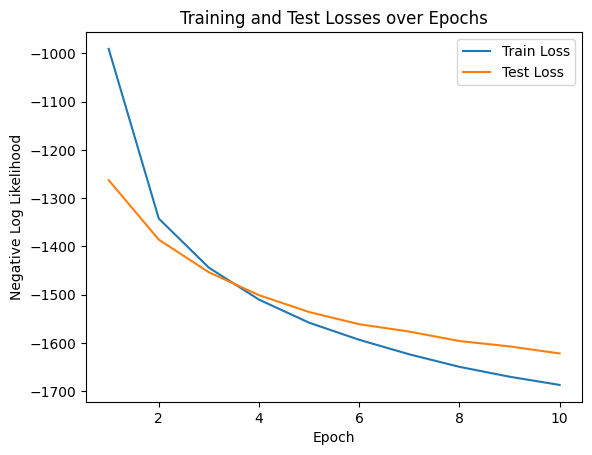
\includegraphics[width=0.8\textwidth]{images/CA2_DGM_cell4_out20.png}
    \caption{Training and validation loss curves for RealNVP model. The negative log-likelihood decreases over epochs, indicating successful learning of the data distribution.}
    \label{fig:realnvp_loss}
\end{figure}

\subsubsection{Generated Samples}

Samples are generated by sampling from the base Gaussian distribution and applying the inverse transformation:

\begin{lstlisting}[caption={Sampling from RealNVP}]
with torch.no_grad():
    z = torch.randn(9, input_dim).to(device)
    x_samples = model.inverse(z)
    x_samples = x_samples.cpu().view(-1, 1, 28, 28)
\end{lstlisting}

\begin{figure}[H]
    \centering
    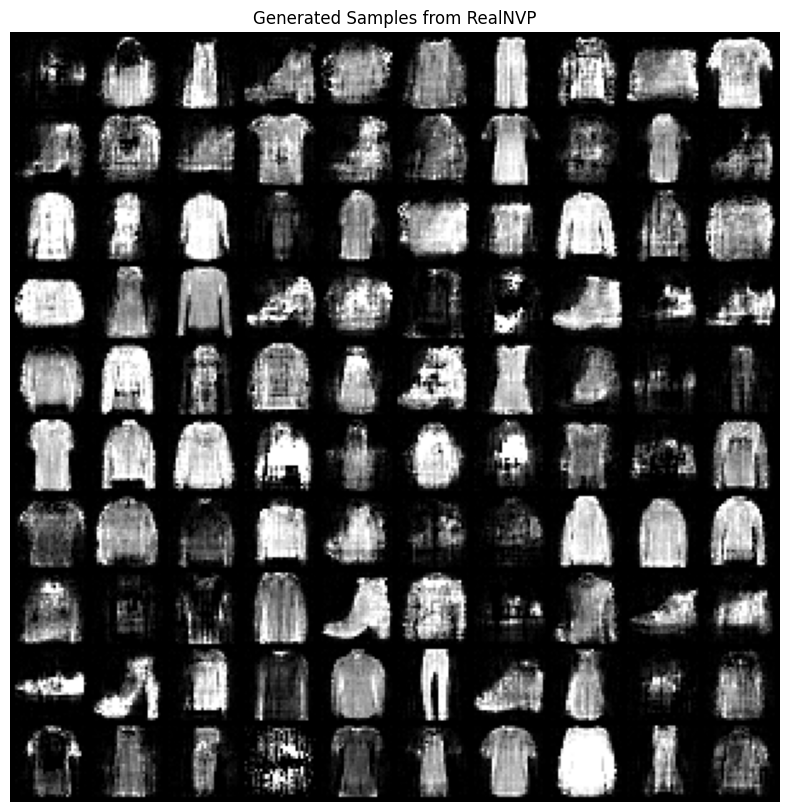
\includegraphics[width=0.6\textwidth]{images/CA2_DGM_cell11_out1.png}
    \caption{Generated FashionMNIST samples from RealNVP model after training. The model learns to generate diverse fashion items with reasonable quality.}
    \label{fig:realnvp_samples}
\end{figure}

\subsection{Out-of-Distribution Detection Using Flow-Based Models (3 points)}

\subsubsection{Probabilistic OOD Detection Method}

Flow-based models enable out-of-distribution (OOD) detection through likelihood evaluation. The key insight is that well-trained flow models assign higher likelihoods to in-distribution data compared to OOD data.

\subsubsection{Methodology}

\begin{enumerate}
    \item \textbf{Train Flow Model}: Train RealNVP on FashionMNIST training data
    \item \textbf{Compute Likelihoods}: Calculate log-likelihoods for:
    \begin{itemize}
        \item FashionMNIST test set (in-distribution)
        \item MNIST test set (OOD - different distribution)
        \item KMNIST test set (OOD - different distribution)
    \end{itemize}
    \item \textbf{Compare Distributions}: Analyze likelihood distributions to identify OOD samples
\end{enumerate}

\subsubsection{Implementation}

\begin{lstlisting}[caption={Log-Likelihood Computation for OOD Detection}]
def compute_log_likelihood(model, data_loader):
    model.eval()
    log_likelihoods = []
    with torch.no_grad():
        for data, _ in data_loader:
            data = data.view(-1, input_dim).to(device)
            z, log_det_jacobian = model(data)
            log_pz = -0.5 * torch.sum(z ** 2 + np.log(2 * np.pi), dim=1)
            log_px = log_pz + log_det_jacobian
            log_likelihoods.append(log_px.cpu().numpy())
    return np.concatenate(log_likelihoods)
\end{lstlisting}

\subsubsection{Results}

The computed log-likelihoods are:

\begin{itemize}
    \item \textbf{FashionMNIST Train}: 1706.93
    \item \textbf{FashionMNIST Test}: 1621.40
    \item \textbf{MNIST}: 890.02 (OOD - lower likelihood)
    \item \textbf{KMNIST}: -1850.95 (OOD - negative likelihood, very different)
\end{itemize}

\begin{figure}[H]
    \centering
    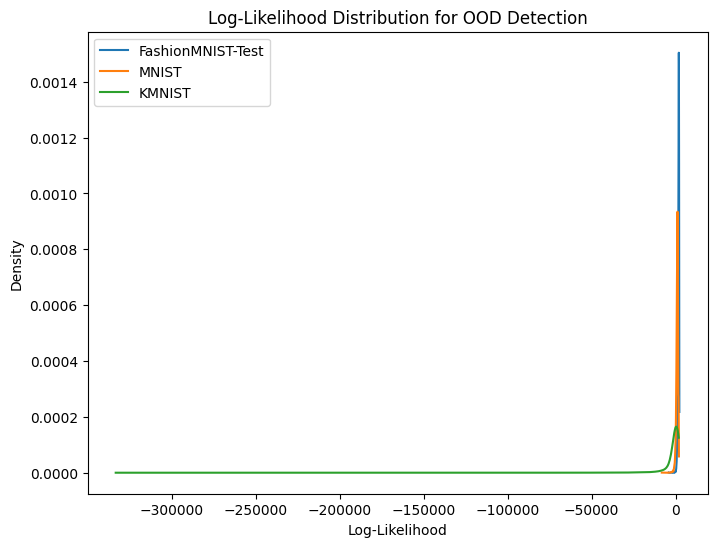
\includegraphics[width=0.7\textwidth]{images/CA2_DGM_cell10_out0.png}
    \caption{Log-likelihood distributions for FashionMNIST test, MNIST, and KMNIST datasets. FashionMNIST has the highest likelihood as expected, while MNIST and KMNIST show lower likelihoods, enabling OOD detection.}
    \label{fig:ood_detection}
\end{figure}

\subsubsection{Limitations of Flow-Based OOD Detection}

\begin{enumerate}
    \item \textbf{Likelihood vs. Quality}: Flow models may assign high likelihoods to background/noise patterns if they dominate the training data
    \item \textbf{Feature Mismatch}: Flow models trained on pixel space may not capture semantic features needed for semantic OOD detection
    \item \textbf{Dimensionality Curse}: High-dimensional data spaces make density estimation challenging, leading to potential overfitting
    \item \textbf{Mode Collapse}: Flow models might not cover all modes of the data distribution, missing some in-distribution patterns
\end{enumerate}

\subsection{Likelihood Evaluation and Analysis (12 points)}

\subsubsection{Pixel Space vs. Latent Space Comparison}

We compare RealNVP performance in two settings:

\begin{enumerate}
    \item \textbf{Pixel Space}: Direct application on flattened 784-dimensional images
    \item \textbf{Latent Space}: Application on learned latent representations (32-dimensional) from an autoencoder
\end{enumerate}

\subsubsection{Latent Space Architecture}

First, we train an encoder-decoder pair to learn a compressed representation:

\begin{lstlisting}[caption={Encoder and Decoder Architecture}]
class Encoder(nn.Module):
    def __init__(self, input_dim, latent_dim):
        super(Encoder, self).__init__()
        self.encoder = nn.Sequential(
            nn.Linear(input_dim, 512),
            nn.ReLU(),
            nn.Linear(512, latent_dim)
        )
    def forward(self, x):
        return self.encoder(x)

class Decoder(nn.Module):
    def __init__(self, latent_dim, output_dim):
        super(Decoder, self).__init__()
        self.decoder = nn.Sequential(
            nn.Linear(latent_dim, 512),
            nn.ReLU(),
            nn.Linear(512, output_dim)
        )
    def forward(self, x):
        return self.decoder(x)
\end{lstlisting}

The autoencoder is trained with MSE reconstruction loss for 5 epochs, achieving train loss of 0.0076.

\subsubsection{Results Comparison}

\textbf{Pixel Space Results:}
\begin{itemize}
    \item FashionMNIST Train Log-Likelihood: 1706.93
    \item FashionMNIST Test Log-Likelihood: 1621.40
    \item MNIST Log-Likelihood: 890.02
    \item KMNIST Log-Likelihood: -1850.95
\end{itemize}

\textbf{Latent Space Results (after encoding):}
\begin{itemize}
    \item FashionMNIST Train Log-Likelihood: 166.30
    \item FashionMNIST Test Log-Likelihood: 151.64
    \item MNIST Log-Likelihood: 2.39
    \item KMNIST Log-Likelihood: -66.17
\end{itemize}

\subsubsection{Analysis}

\begin{enumerate}
    \item \textbf{Better Separation}: In latent space, the separation between in-distribution and OOD data is more pronounced (FashionMNIST: 151.64 vs MNIST: 2.39 vs KMNIST: -66.17)
    
    \item \textbf{Computational Efficiency}: Working in 32-dimensional latent space is significantly more efficient than 784-dimensional pixel space
    
    \item \textbf{Semantic Features}: The autoencoder learns semantic features that better distinguish between different datasets
    
    \item \textbf{OOD Detection Improvement}: The relative difference between FashionMNIST and OOD datasets is larger in latent space, making OOD detection more reliable
\end{enumerate}

\subsection{Hidden Space Experiments (6 points)}

The latent space experiments demonstrate that applying normalizing flows in learned latent representations provides several advantages:

\begin{enumerate}
    \item \textbf{Reduced Dimensionality}: Working with 32-D latent codes instead of 784-D pixels reduces computational complexity
    
    \item \textbf{Better Feature Extraction}: The encoder learns meaningful features that better represent the data distribution
    
    \item \textbf{Improved OOD Detection}: The likelihood gap between in-distribution and OOD data is more significant in latent space
    
    \item \textbf{Faster Training}: RealNVP training converges faster in the lower-dimensional latent space
\end{enumerate}

\subsubsection{Training Loss Comparison}

\begin{itemize}
    \item \textbf{Pixel Space}: Negative log-likelihood values around 1700-1600
    \item \textbf{Latent Space}: Negative log-likelihood values around -150 to -160 (higher is better for likelihood)
\end{itemize}

The latent space model achieves negative log-likelihood of -164.52 after 10 epochs, showing excellent density modeling performance.

\newpage

\section{Question 2: Generative Adversarial Networks (GANs)}

\subsection{Analysis of GAN Training Objectives (5 points)}

Generative Adversarial Networks (GANs) are trained through a minimax game between two neural networks: a generator $G$ and a discriminator $D$.

\subsubsection{Objective Functions}

The GAN objective function is formulated as a two-player minimax game:

\begin{equation}
    \min_G \max_D V(D, G) = \mathbb{E}_{x \sim p_{data}(x)}[\log D(x)] + \mathbb{E}_{z \sim p_z(z)}[\log(1-D(G(z)))]
\end{equation}

Where:
\begin{itemize}
    \item $p_{data}(x)$: Real data distribution
    \item $p_z(z)$: Prior distribution over noise (typically $\mathcal{N}(0, I)$)
    \item $G(z)$: Generator mapping noise to data space
    \item $D(x)$: Discriminator output (probability that $x$ is real)
\end{itemize}

\subsubsection{Separate Loss Functions}

\textbf{Discriminator Loss:}
\begin{equation}
    L_D(\phi; \theta) = - \mathbb{E}_{x \sim p_{data}(x)}[\log D_\phi(x)] - \mathbb{E}_{z \sim \mathcal{N}(0,1)}[\log(1 - D_\phi(G_\theta(z)))]
\end{equation}

The discriminator aims to \textit{maximize} this, which means:
\begin{itemize}
    \item Maximize $\log D(x)$ for real samples (increase probability of real)
    \item Maximize $\log(1-D(G(z)))$ for fake samples (increase probability of fake)
\end{itemize}

\textbf{Generator Loss:}
\begin{equation}
    L_G(\phi; \theta) = \mathbb{E}_{z \sim \mathcal{N}(0,1)}[\log(1 - D_\phi(G_\theta(z)))]
\end{equation}

The generator aims to \textit{minimize} this, which means making $D(G(z))$ as large as possible (fooling the discriminator).

\subsubsection{Vanishing Gradients Problem}

The generator loss $L_G = \mathbb{E}[\log(1-D(G(z)))]$ suffers from vanishing gradients when the discriminator is near optimal. Here's why:

\begin{enumerate}
    \item \textbf{When $D$ is optimal}: $D^*(x) = \frac{p_{data}(x)}{p_{data}(x) + p_\theta(x)}$
    
    \item \textbf{Poor generator}: If $p_\theta(x) \approx 0$ (generator produces bad samples), then $D^*(G(z)) \approx 0$
    
    \item \textbf{Gradient computation}: The gradient of generator loss is:
    \begin{equation}
        \nabla_\theta L_G = \mathbb{E}_{z} \left[ \frac{D'(G_\theta(z))}{1-D(G_\theta(z))} \nabla_\theta G_\theta(z) \right]
    \end{equation}
    
    \item \textbf{Problem}: When $D(G(z)) \approx 0$, we have:
    \begin{itemize}
        \item $\log(1-D(G(z))) \approx \log(1-0) = 0$ (saturated)
        \item The gradient $\frac{\partial L_G}{\partial \theta}$ becomes very small (vanishing)
        \item Generator learns slowly or stops learning
    \end{itemize}
\end{enumerate}

\subsubsection{Impact on Training}

The vanishing gradients issue causes:
\begin{itemize}
    \item \textbf{Slow convergence}: Generator makes little progress when discriminator is strong
    \item \textbf{Training instability}: Oscillations between generator and discriminator
    \item \textbf{Non-convergence}: Generator may fail to learn the data distribution
\end{itemize}

\subsubsection{Solution: Non-Saturating Loss}

A common solution is to use the \textbf{non-saturating generator loss}:
\begin{equation}
    L_G^{non-sat} = - \mathbb{E}_{z \sim \mathcal{N}(0,1)}[\log(D(G(z)))]
\end{equation}

This loss provides stronger gradients when $D(G(z))$ is small, encouraging the generator to improve even when the discriminator is strong.

\subsection{Optimal Discriminator Derivation (5 points)}

For a fixed generator $G$, we derive the optimal discriminator $D^*$ that maximizes $V(D,G)$.

\subsubsection{Derivation}

The discriminator objective is:
\begin{equation}
    V(D, G) = \mathbb{E}_{x \sim p_{data}}[\log D(x)] + \mathbb{E}_{z \sim p_z}[\log(1-D(G(z)))]
\end{equation}

Rewriting in terms of $x \sim p_{data}$ and $\tilde{x} = G(z) \sim p_\theta$:
\begin{equation}
    V(D, G) = \int p_{data}(x) \log D(x) dx + \int p_\theta(x) \log(1-D(x)) dx
\end{equation}

For a fixed point $x$, we maximize $f(D(x)) = p_{data}(x) \log D(x) + p_\theta(x) \log(1-D(x))$ with respect to $D(x)$.

Taking the derivative:
\begin{equation}
    \frac{\partial f}{\partial D(x)} = \frac{p_{data}(x)}{D(x)} - \frac{p_\theta(x)}{1-D(x)} = 0
\end{equation}

Solving for $D(x)$:
\begin{align}
    \frac{p_{data}(x)}{D(x)} &= \frac{p_\theta(x)}{1-D(x)} \\
    p_{data}(x)(1-D(x)) &= p_\theta(x) D(x) \\
    p_{data}(x) - p_{data}(x) D(x) &= p_\theta(x) D(x) \\
    p_{data}(x) &= D(x)(p_{data}(x) + p_\theta(x)) \\
    D^*(x) &= \frac{p_{data}(x)}{p_{data}(x) + p_\theta(x)}
\end{align}

\subsubsection{Optimal Discriminator Loss}

Substituting $D^*(x)$ back into the objective:
\begin{align}
    V(D^*, G) &= \mathbb{E}_{x \sim p_{data}} \left[ \log \frac{p_{data}(x)}{p_{data}(x) + p_\theta(x)} \right] \\
    &\quad + \mathbb{E}_{x \sim p_\theta} \left[ \log \frac{p_\theta(x)}{p_{data}(x) + p_\theta(x)} \right]
\end{align}

This can be rewritten as:
\begin{align}
    V(D^*, G) &= \mathbb{E}_{x \sim p_{data}} \left[ \log \frac{2p_{data}(x)}{p_{data}(x) + p_\theta(x)} \right] - \log 2 \\
    &\quad + \mathbb{E}_{x \sim p_\theta} \left[ \log \frac{2p_\theta(x)}{p_{data}(x) + p_\theta(x)} \right] - \log 2 \\
    &= 2 \cdot \text{JSD}(p_{data} \| p_\theta) - 2\log 2
\end{align}

\subsubsection{Relation to Jensen-Shannon Divergence}

The Jensen-Shannon Divergence (JSD) between two distributions $P$ and $Q$ is:
\begin{equation}
    \text{JSD}(P \| Q) = \frac{1}{2} \text{KL}\left(P \| \frac{P+Q}{2}\right) + \frac{1}{2} \text{KL}\left(Q \| \frac{P+Q}{2}\right)
\end{equation}

Therefore:
\begin{equation}
    \min_G V(D^*, G) = \min_G 2 \cdot \text{JSD}(p_{data} \| p_\theta) - 2\log 2
\end{equation}

This shows that:
\begin{itemize}
    \item Training GANs is equivalent to minimizing JSD between real and generated distributions
    \item The global minimum occurs when $p_\theta = p_{data}$ (generator perfectly matches data)
    \item At optimality, $D^*(x) = \frac{1}{2}$ for all $x$ (discriminator cannot distinguish real from fake)
\end{itemize}

\subsection{Discriminator Logit Relationship (3 points)}

\subsubsection{Discriminator Output Structure}

The discriminator outputs a probability via a sigmoid:
\begin{equation}
    D_\phi(x) = \sigma(h_\phi(x)) = \frac{1}{1 + \exp(-h_\phi(x))}
\end{equation}

where $h_\phi(x)$ is the logit (pre-sigmoid output).

\subsubsection{Optimal Logit Derivation}

When $D_\phi = D^*$, we have:
\begin{equation}
    D^*(x) = \sigma(h^*(x)) = \frac{p_{data}(x)}{p_{data}(x) + p_\theta(x)}
\end{equation}

Solving for $h^*(x)$:
\begin{align}
    \frac{1}{1 + \exp(-h^*(x))} &= \frac{p_{data}(x)}{p_{data}(x) + p_\theta(x)} \\
    1 + \exp(-h^*(x)) &= \frac{p_{data}(x) + p_\theta(x)}{p_{data}(x)} \\
    \exp(-h^*(x)) &= \frac{p_\theta(x)}{p_{data}(x)} \\
    h^*(x) &= -\log \frac{p_\theta(x)}{p_{data}(x)} \\
    h^*(x) &= \log \frac{p_{data}(x)}{p_\theta(x)}
\end{align}

\subsubsection{Interpretation}

The optimal discriminator logit $h^*(x) = \log \frac{p_{data}(x)}{p_\theta(x)}$ represents:

\begin{itemize}
    \item \textbf{Log-Density Ratio}: The logarithm of the ratio between real data density and generated data density
    
    \item \textbf{Classification Signal}: 
    \begin{itemize}
        \item If $p_{data}(x) > p_\theta(x)$, then $h^*(x) > 0$ and $D^*(x) > 0.5$ (classified as real)
        \item If $p_{data}(x) < p_\theta(x)$, then $h^*(x) < 0$ and $D^*(x) < 0.5$ (classified as fake)
        \item If $p_{data}(x) = p_\theta(x)$, then $h^*(x) = 0$ and $D^*(x) = 0.5$ (uncertain)
    \end{itemize}
    
    \item \textbf{Optimality Indicator}: When the generator is optimal ($p_\theta = p_{data}$), $h^*(x) = 0$ for all $x$, meaning the discriminator is maximally confused
\end{itemize}

\subsection{WGAN and Its Benefits (5 points)}

Wasserstein GAN (WGAN) addresses critical issues in traditional GANs by replacing Jensen-Shannon divergence with Wasserstein distance.

\subsubsection{Wasserstein Distance}

The Wasserstein-1 (or Earth Mover's) distance between two distributions $p_r$ and $p_\theta$ is:
\begin{equation}
    W(p_r, p_\theta) = \inf_{\gamma \in \Pi(p_r, p_\theta)} \mathbb{E}_{(x,y) \sim \gamma} [\|x-y\|]
\end{equation}

where $\Pi(p_r, p_\theta)$ is the set of all joint distributions with marginals $p_r$ and $p_\theta$.

Using Kantorovich-Rubinstein duality:
\begin{equation}
    W(p_r, p_\theta) = \sup_{\|f\|_L \leq 1} \left[ \mathbb{E}_{x \sim p_r}[f(x)] - \mathbb{E}_{x \sim p_\theta}[f(x)] \right]
\end{equation}

where $\|f\|_L \leq 1$ denotes that $f$ is 1-Lipschitz.

\subsubsection{WGAN Objective}

WGAN replaces the discriminator with a critic $f$ (1-Lipschitz function):
\begin{equation}
    \min_G \max_{\|f\|_L \leq 1} \left[ \mathbb{E}_{x \sim p_r}[f(x)] - \mathbb{E}_{z \sim p_z}[f(G(z))] \right]
\end{equation}

\subsubsection{Benefits of WGAN}

\begin{enumerate}
    \item \textbf{Solves Vanishing Gradients}: 
    \begin{itemize}
        \item Wasserstein distance is continuous and differentiable almost everywhere
        \item Provides meaningful gradients even when distributions have disjoint support
        \item Generator can learn even when critic is near optimal
    \end{itemize}
    
    \item \textbf{Improved Convergence}:
    \begin{itemize}
        \item Wasserstein distance correlates better with generation quality
        \item Training is more stable and predictable
        \item Lower risk of mode collapse
    \end{itemize}
    
    \item \textbf{Better Distance Metric}:
    \begin{itemize}
        \item JS divergence can be infinite even for similar distributions
        \item Wasserstein distance is always finite and continuous
        \item Better reflects perceptual similarity
    \end{itemize}
\end{enumerate}

\subsubsection{Lipschitz Constraint Implementation}

To enforce $\|f\|_L \leq 1$, WGAN uses:

\textbf{Weight Clipping} (original WGAN):
\begin{itemize}
    \item Clip all critic weights to a fixed interval $[-c, c]$ (e.g., $c = 0.01$)
    \item Simple but can limit model capacity
    \item May cause optimization issues
\end{itemize}

\textbf{Gradient Penalty} (WGAN-GP):
\begin{itemize}
    \item Adds a penalty term to enforce 1-Lipschitz constraint:
    \begin{equation}
        \lambda \mathbb{E}_{\hat{x} \sim p_{\hat{x}}} \left[ (\|\nabla_{\hat{x}} f(\hat{x})\|_2 - 1)^2 \right]
    \end{equation}
    where $\hat{x}$ is sampled along straight lines between real and generated samples
    \item More flexible and stable than weight clipping
    \item Better gradient flow
\end{itemize}

\subsubsection{Comparison: Traditional GAN vs WGAN}

\begin{table}[H]
\centering
\begin{tabular}{|l|p{5cm}|p{5cm}|}
\hline
\textbf{Aspect} & \textbf{Traditional GAN} & \textbf{WGAN} \\
\hline
Distance Metric & JS Divergence & Wasserstein Distance \\
\hline
Gradient Stability & Vanishing when D optimal & Meaningful gradients always \\
\hline
Training Stability & Often unstable & More stable \\
\hline
Architecture & Requires specific design & More flexible architectures \\
\hline
Mode Collapse & Common problem & Reduced tendency \\
\hline
\end{tabular}
\caption{Comparison between Traditional GANs and WGAN}
\label{tab:gan_comparison}
\end{table}

\subsection{Evaluation Metrics for GAN Convergence (4 points)}

Evaluating GAN performance is challenging because explicit likelihood computation is not available. Several metrics have been developed:

\subsubsection{Fréchet Inception Distance (FID)}

FID measures the distance between feature distributions of real and generated images using a pre-trained Inception network.

\textbf{Mathematical Formulation:}

\begin{equation}
    \text{FID} = \|\mu_r - \mu_g\|^2 + \text{Tr}(\Sigma_r + \Sigma_g - 2(\Sigma_r \Sigma_g)^{1/2})
\end{equation}

Where:
\begin{itemize}
    \item $\mu_r, \Sigma_r$: Mean and covariance of real image features
    \item $\mu_g, \Sigma_g$: Mean and covariance of generated image features
    \item Features extracted from Inception v3 network (2048-dimensional)
\end{itemize}

\textbf{Advantages:}
\begin{itemize}
    \item Correlates well with human perception
    \item Sensitive to mode collapse (low diversity)
    \item Works well for high-dimensional distributions
    \item Standardized metric for comparison
\end{itemize}

\textbf{Interpretation:}
\begin{itemize}
    \item Lower FID = Better quality (typical ranges: <50 excellent, 50-100 good, >200 poor)
    \item Captures both quality and diversity
    \item Requires Inception network computation (more expensive than IS)
\end{itemize}

\subsubsection{Wasserstein Distance}

Direct Wasserstein distance between real and generated distributions:

\begin{itemize}
    \item \textbf{Computation}: Can be estimated using optimal transport
    \item \textbf{Benefits}: Mathematically principled, continuous metric
    \item \textbf{Limitations}: Computationally expensive for high-dimensional data
    \item \textbf{Usage}: More theoretical than practical for evaluation
\end{itemize}

\subsubsection{Visual Quality Assessment}

Qualitative evaluation through visual inspection:

\begin{itemize}
    \item \textbf{Sample Quality}: Are generated images realistic and sharp?
    \item \textbf{Diversity}: Do samples cover various modes of the distribution?
    \item \textbf{Mode Coverage}: Are all classes/styles represented?
    \item \textbf{Artifacts}: Presence of mode collapse, artifacts, or repetitive patterns
\end{itemize}

\subsubsection{Inception Score (IS)}

\begin{equation}
    \text{IS}(G) = \exp\left( \mathbb{E}_{x \sim p_g} [\text{KL}(p(y|x) \| p(y))] \right)
\end{equation}

Where:
\begin{itemize}
    \item $p(y|x)$: Classifier prediction distribution
    \item $p(y)$: Marginal class distribution
    \item Measures both quality and diversity
\end{itemize}

\textbf{Limitations:}
\begin{itemize}
    \item Requires class labels (not always available)
    \item Can be fooled by memorization
    \item Less reliable than FID for many applications
\end{itemize}

\subsubsection{Practical Evaluation Strategy}

For our FashionMNIST GAN implementation, we use:

\begin{enumerate}
    \item \textbf{FID Scores}: Computed after each epoch using pytorch-fid
    \item \textbf{Loss Curves}: Monitor generator and discriminator losses
    \item \textbf{Visual Inspection}: Generate sample grids to assess quality and diversity
    \item \textbf{Training Stability}: Monitor for oscillations, mode collapse, or divergence
\end{enumerate}

\newpage

